%************************************************
\chapter{Introduction}
\label{chapter:introduction}
%************************************************

\begin{figure}[bth]
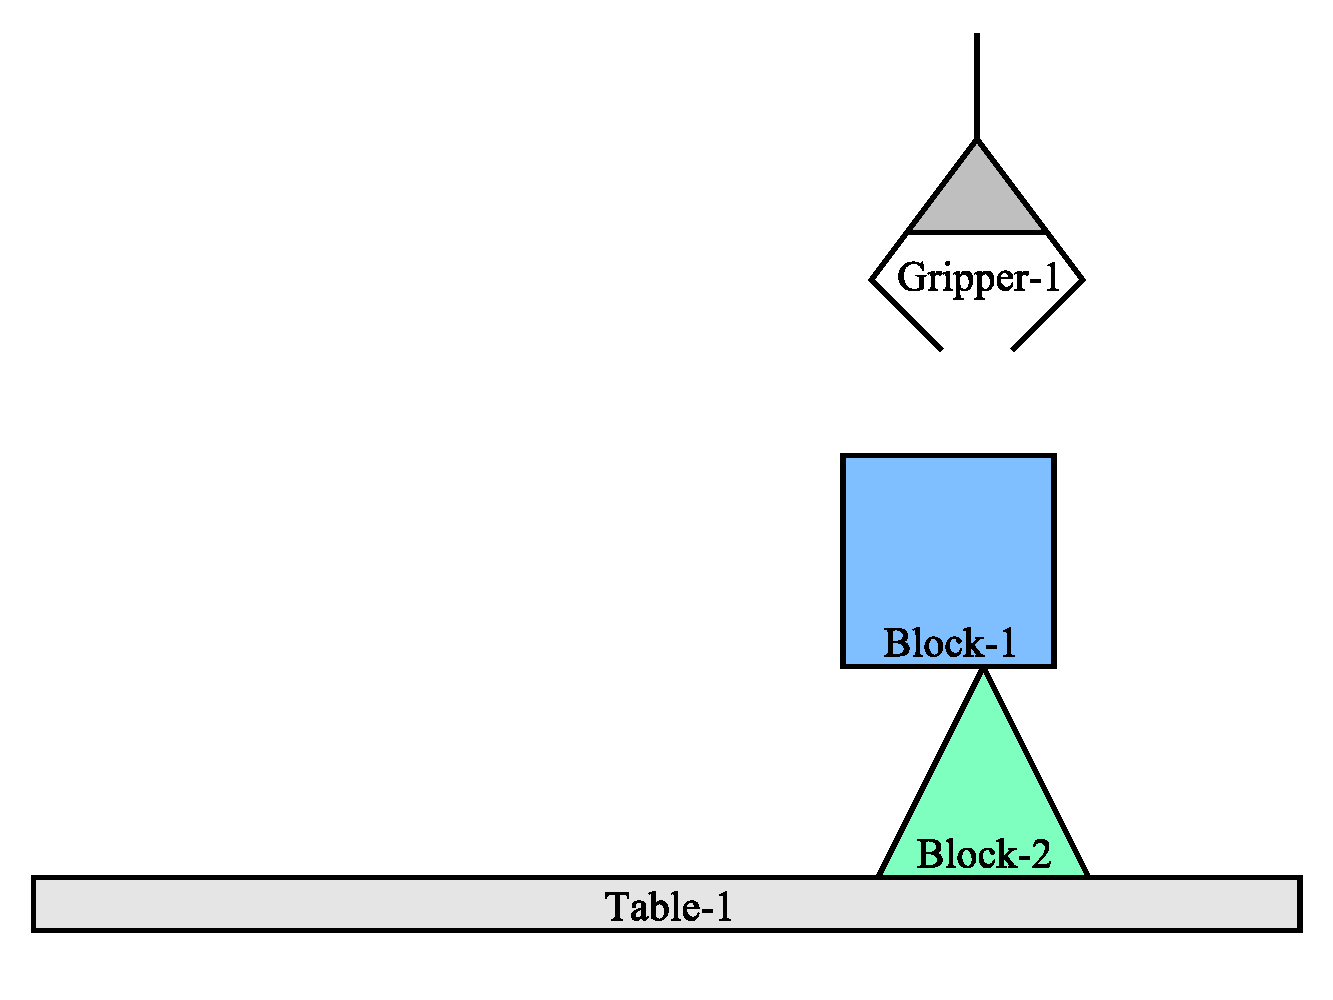
\includegraphics[width=10cm]{gfx/blocks_world_example_failure} \\ \medskip
\caption{A failure to stack two blocks.}
\label{figure:example_of_failure}
\end{figure}

My thesis is SALS, a computational simulation of a model of learning
in multiple reflective layers.  I begin my explanation with a
description of the example situation pictured in
\autoref{figure:example_of_failure}:
\begin{quote}
There is a table.  Some blocks are on the table.  The blocks are of
different shapes and colors.  One of the blocks is a green triangle.
Another block is a blue square.  A gripper can move around, picking up
and putting down blocks.  Plans are made for the gripper to arrange
the blocks into different configurations.  Plans are followed that
sometimes result in a failure.  For example, putting the square on top
of the triangle fails to stack the two blocks because the square falls
off of the triangle.  A single failure is a learning opportunity.  A
better model of the world can be learned through each failure.
\end{quote}
This is a common type of situation for current learning algorithms,
updating models of the world when experiences fail to match
expectations.  What I show in this thesis is that better models of
planning strategies can also be learned from these same failures.
Learning different planning strategies for different situations is a
reflective form of thinking.  Thus, my thesis is SALS, which provides
a working example of turning a single failure into failures at
multiple reflective layers, demonstrating multiple learning
opportunities from a single failure.

I begin with a non-technical description of the model in plain
English.  At the end of \autoref{part:the_model}, I explain the
modelling assumptions that I make in transitioning to the mathematical
notation of \autoref{part:simulating_the_model}.  Using this notation,
I explain how this model can be used to reduce the complexity of
search algorithms.  In \autoref{part:the_implementation}, I give an
explanation of how this simulation is automated on a concurrent
computer, the thesis implementation, SALS, the substrate for
accountable layered systems.  In conclusion, in
\autoref{part:conclusion}, I discuss promising directions for future
research in not only AI but also the other cognitive sciences.

\section{Motivation}

\section{Explanation of the Problem}

\section{Contributions}

\section{Document Overview}

